% ======================================================================
%  Personal LaTeX Template
%  Victor Gabriele De Matteis
%
%  Citation style: numeric [1], compact (abbrvnat).
%  To switch to author-year, replace:
%    \usepackage[numbers,square,sort&compress]{natbib}
%    \bibliographystyle{abbrvnat}
%  with:
%    \usepackage[round,authoryear]{natbib}
%    \bibliographystyle{apalike}
% ======================================================================

\documentclass[10pt,a4paper]{scrartcl}

% --------------------------------------------------
% Encoding and language
% --------------------------------------------------
\usepackage[T1]{fontenc}
\usepackage[utf8]{inputenc}
\usepackage[english]{babel}

% --------------------------------------------------
% Page layout
% --------------------------------------------------
\usepackage[
top=10mm,
bottom=10mm,
left=20mm,
right=20mm,
includefoot
]{geometry}
\usepackage{multicol}

\setlength{\columnsep}{8mm}      % distance between columns
\setlength{\columnseprule}{0pt}  % no vertical rule

% --------------------------------------------------
% Mathematics and graphics
% --------------------------------------------------
\usepackage{graphicx}
\usepackage{subcaption}
\usepackage{wrapfig}
\usepackage{mathtools} % loads amsmath automatically
%\usepackage{amssymb}
\usepackage{bm}

% Let figures pack densely with text instead of drifting to float pages.
\renewcommand{\topfraction}{0.92}
\renewcommand{\bottomfraction}{0.85}
\renewcommand{\textfraction}{0.06}
\renewcommand{\floatpagefraction}{0.75}
\setcounter{topnumber}{3}
\setcounter{totalnumber}{4}

% --------------------------------------------------
% Tables
% --------------------------------------------------
\usepackage{booktabs}
\usepackage{tabularx}
\usepackage{array}
\usepackage{ragged2e}

% A ragged-right fixed-width column for use in tabularx:
%   \begin{tabularx}{\textwidth}{@{}L{3cm} X@{}}
\newcolumntype{L}[1]{>{\RaggedRight\arraybackslash}p{#1}}

% --------------------------------------------------
% Typography
% --------------------------------------------------
\usepackage[scaled=0.95]{helvet}
\usepackage[expansion=false]{microtype}   % expansion=false avoids font errors
\renewcommand{\familydefault}{\sfdefault} % sans-serif throughout

% --------------------------------------------------
% Lists
% --------------------------------------------------
\usepackage{enumitem}
\setlist[itemize]{
leftmargin=*,
topsep=2pt,
parsep=0pt,
partopsep=0pt,
itemsep=3pt
}
\setlist[description]{
leftmargin=0pt,
topsep=2pt,
parsep=0pt,
itemsep=3pt
}

% --------------------------------------------------
% Colour and hyperlinks
% --------------------------------------------------
\usepackage[dvipsnames]{xcolor}
\usepackage[hidelinks]{hyperref}

\definecolor{accent}{RGB}{25,55,140}   % change this to restyle everything

% --- tinted, rounded, fixed-padding panel behind figures (image + caption) ---
%\definecolor{figbg}{RGB}{247,247,243}          % dirty white
\colorlet{figbg}{accent!7!white}  % 7% accent, 93% white
\usepackage[most]{tcolorbox}
\newtcolorbox{figpanelenv}[1]{%  #1 = outer width
  colback=figbg, colframe=figbg, boxrule=0pt,
  arc=4pt,                                   % corner radius
  boxsep=0pt, left=6pt, right=6pt, top=6pt, bottom=6pt,  % fixed padding
  width=#1, halign=center,
  before skip=0pt, after skip=0pt
}

% \emph produces upright accent-coloured text instead of italic.
% Use \textit{} when you genuinely want italics.
\renewcommand{\emph}[1]{\textit{#1}}

% --------------------------------------------------
% Citations
% --------------------------------------------------
\usepackage[numbers,square,sort&compress]{natbib}

% --------------------------------------------------
% Header and footer
% --------------------------------------------------
\usepackage[automark,headsepline=false,footsepline=false]{scrlayer-scrpage}
\clearpairofpagestyles

%  Edit the three footer fields below:
\ifoot{Victor Gabriele De Matteis}          % left:   your name / student ID
\cfoot{\pagemark}            % centre: page number (always keep this)
\ofoot{AC Course Project 2025/2026}    % right:  course name or document label

\setlength{\footskip}{15mm}  % pushes footer toward the page edge
\pagestyle{scrheadings}

% --------------------------------------------------
% Spacing
% --------------------------------------------------
%\setlength{\parindent}{0pt}
%\setlength{\parskip}{0.45em}

% --------------------------------------------------
% Section formatting
% --------------------------------------------------
\RedeclareSectionCommand[
beforeskip=1.4ex plus 0.2ex minus 0.1ex,
afterskip=0.6ex
]{section}
\RedeclareSectionCommand[
beforeskip=1.0ex plus 0.2ex minus 0.1ex,
afterskip=0.4ex
]{subsection}
\RedeclareSectionCommand[
beforeskip=0.7ex plus 0.2ex minus 0.1ex,
afterskip=0.3ex
]{subsubsection}

\setkomafont{section}{\large\bfseries\color{accent}}
\setkomafont{subsection}{\normalsize\bfseries\color{accent}}
\setkomafont{subsubsection}{\normalsize\bfseries}

% A section command that adds a faint rule beneath the title.
% Use \RuleSection{Title} instead of \section{Title} where you want it.
\newcommand{\RuleSection}[1]{%
\section{#1}%
\vspace{0.2em}{\color{accent!35}\hrule height 0.4pt}\vspace{0.3em}%
}

% ======================================================================
\begin{document}
% ======================================================================

% --------------------------------------------------
% Title block
% --------------------------------------------------
\begin{center}
{\Large\bfseries\color{accent} Automatic Control Course Project}\\[0.25cm]
{\small Università di Trento --- Automatic Control --- A.Y.\ 2025/2026 $\qquad\qquad$}
{\small Victor Gabriele De Matteis, ID. 265757}\\[0.2cm]
\end{center}


% ======================================================================
%  BODY
% ======================================================================


\RuleSection{Introduction}
\label{sec:intro}

All the constructions in this report are carried out on a linear model obtained by linearizing the dynamics about an equilibrium $(\bar x, \bar u)$, so all coordinates are expressed in deviation variables 

$$\delta x = x - \bar x, \qquad \delta u = u - \bar u, \qquad \delta\omega = \omega - \bar\omega,$$

therefore, every gain, estimate and response that follows is understood relative to this operating point. 
Absolute quantities are recovered as  $x = \bar x + \delta x$ and $u = \bar u + \delta u$.

\RuleSection{Modelling and Linearization}
\label{sec:q1}

\subsection{Operating point}

The steady state conditions $\dot h_1 = \dot h_2=0$ provide two algebraic equations in five unknowns, so the admissible equilibria form a three-parameter family. The operating point therefore is a design choice rather than a property fixed by the plant. 

We linearise about $\bar h_1 = \bar h_2 = 0.2$ m, the maximum admissible level and therefore the most demanding steady state the closed loop is required to hold. 
Fixing the two levels leaves us with one parameter: $u_2$, upon which both $u_1$ and $u_3$ depend:

\begin{equation}
    \bar u_1=u_2\,\frac{a_2\varphi_1}{q_0},\qquad
    \bar u_3=u_2\,\frac{a_2\varphi_1}{a_3\varphi_2},\qquad
    \varphi_i=\sqrt{2g\,\bar h_i}.
    \label{eq:q1_balance}
\end{equation}

\begin{wrapfigure}{r}{6.4cm}
    \centering
    \begin{figpanelenv}{6.4cm}%
%
    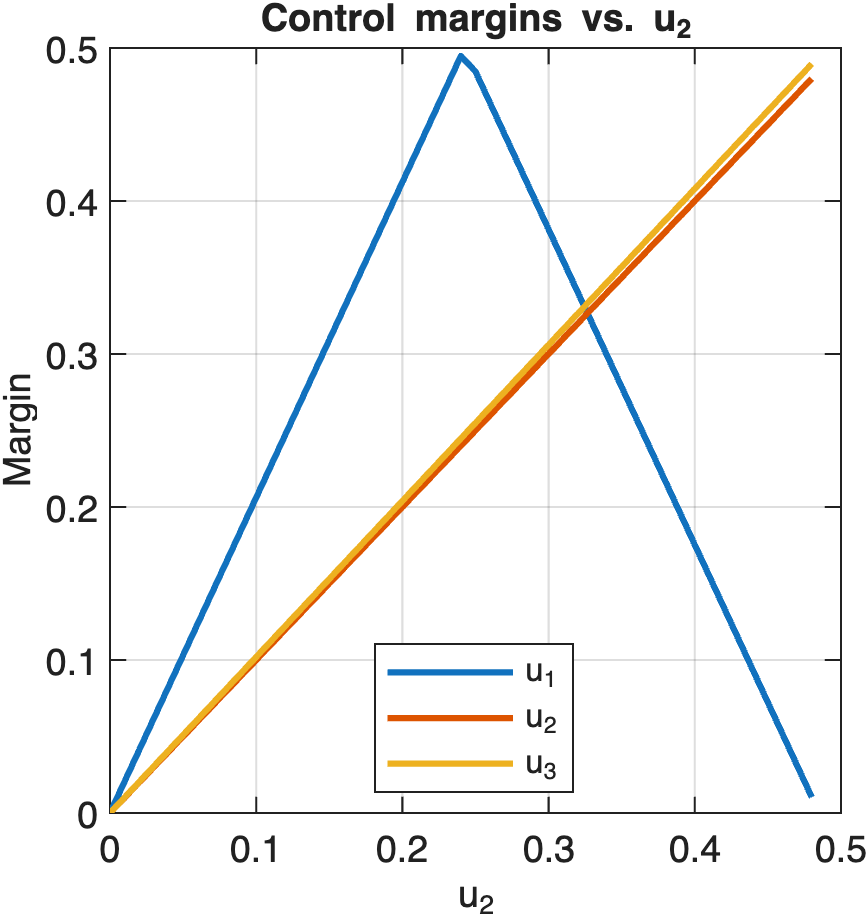
\includegraphics[width=5.7cm]{figures/find_u2}
    \captionof{figure}{\small Actuator margins $\min(\bar u_i,\,1-\bar u_i)$ against the free parameter $u_2$, with $\bar u_1,\bar u_3$ set by the steady-state balance~\eqref{eq:q1_balance}. }
    \label{fig:q1_margins}
    \end{figpanelenv}
\end{wrapfigure}

We resolve this last freedom from the margin sweep of Figure \ref{fig:q1_margins}. Controller margins will become especially important in the next sections, where all inputs will be bounded also during the transient dynamics. The most balanced choice is considered to be the point where these curves cross, it's the best compromise among controller margins. This occurs at $u_2 \approx 0.32$, which we adopt. 

For the operating point, the leakages are set to their nominal healthy-plant value $\bm{\bar \omega} = 0$  for two reasons. First: with the prescribed values for leakages, the equilibrium $\bar h_1 = 0.2$ is not feasible given capping of controllers, as the following calculation demonstrates: 

$$\bar u_1 = \frac{[u_2 a_2 + \alpha_1(h_1 = 0.2)]\,\varphi_1}{q_0} = 1.06 > 1.$$

Furthermore, $\omega$ leaks are framed as disturbances, not as operating conditions, therefore it's not logical to find an equilibrium considering any different value for $\bm{\bar \omega}$, even if mathematically possible. The resulting equilibrium is the following: 
\begin{equation}
    \bar{\bm{x}}=\begin{bmatrix}0.200\\0.200\end{bmatrix}\!\text{m},\qquad
    \bar{\bm{u}}=\begin{bmatrix}0.660\\0.320\\0.326\end{bmatrix}.
    \label{eq:q1_eqpoint}
\end{equation}

\subsection{Linearized model}

Collecting the two balances, the plant follows the following ODEs: 

\begin{equation}
    \dot h_1 = \frac{1}{A_1}\big[\,u_1 q_0 - u_2 a_2\,\varphi_1
                 - \alpha_1\varphi_1\,\big],
    \qquad
    \dot h_2 = \frac{1}{A_2}\big[\,u_2 a_2\,\varphi_1 - u_3 a_3\,\varphi_2
                 - \alpha_2\varphi_2\,\big],
    \label{eq:q1_nl}
\end{equation}

with outflow velocity $\varphi_i \equiv \varphi(h_i) = \sqrt{2 \ g \ h_i}$. Writing $\bm f = [\dot h_1, \dot h_2]^\top$ as a function of $(\bm x, \bm u, \bm \omega)$, the linearised model is obtained from its Jacobians at the operating point, evaluated at our chosen equilibrium:

\begin{equation}
    A=\left.\frac{\partial\bm{f}}{\partial\bm{x}}\right|_\star,\quad
    B=\left.\frac{\partial\bm{f}}{\partial\bm{u}}\right|_\star,\quad
    E=\left.\frac{\partial\bm{f}}{\partial\bm{\omega}}\right|_\star,
    \label{eq:q1_jac}
\end{equation}

The only nonlinearity is $\varphi_i$, whose derivative at the operating level is: 


\begin{equation}
    \beta_i:=\frac{\mathrm{d}\varphi_i}{\mathrm{d}h_i}
    =\frac{g}{\varphi_i}=\frac{g}{\Big({2g\,\bar h_i}\Big)^{1/2}} .
    \label{eq:q1_beta}
\end{equation}

Since the inputs and disturbances enter \eqref{eq:q1_nl} linearly, the entries of $B$ and $E$ are read directly from the coefficients of $\bm u$ and $\bm \omega$, whereas $A$ alone carries the derivative $\beta_i$ through the chain rule. For $\dot h_1$ and analogously for $\dot h_2$, the following holds: 

\begin{equation}
    \frac{\partial\dot h_1}{\partial h_1}
    =-\frac{(u_2a_2+\alpha_1)\,\beta_1}{A_1}
    \;\xrightarrow{\ \bar{\bm{\omega}}=0\ }\;
    -\frac{u_2a_2\,\beta_1}{A_1},\qquad
    \frac{\partial\dot h_1}{\partial u_1}=\frac{q_0}{A_1},\qquad
    \frac{\partial\dot h_1}{\partial\alpha_1}=-\frac{\varphi_1}{A_1},
    \label{eq:q1_entries}
\end{equation}

Evaluating each matrix at the operating point yields the following matrices: 

\begin{equation}
    A=\begin{bmatrix}
        -\dfrac{u_2a_2\beta_1}{A_1} & 0\\[.2cm]
        \phantom{-}\dfrac{u_2a_2\beta_1}{A_2} & -\dfrac{u_3a_3\beta_2}{A_2}
      \end{bmatrix},\qquad
    B=\begin{bmatrix}
        \dfrac{q_0}{A_1} & -\dfrac{a_2\varphi_1}{A_1} & 0\\[.2cm]
        0 & \dfrac{a_2\varphi_1}{A_2} & -\dfrac{a_3\varphi_2}{A_2}
      \end{bmatrix},
    \label{eq:q1_A}
\end{equation}
\begin{equation}
    E=\begin{bmatrix}
        -\dfrac{\varphi_1}{A_1} & 0\\[.2cm]
        0 & -\dfrac{\varphi_2}{A_2}
      \end{bmatrix},\qquad
    C=I_2,\qquad D=0_{2\times3},\qquad F=0_{2\times2}.
    \label{eq:q1_B}
\end{equation}

The numerical values of $A$, $B$, $C$, $D$, $E$ and $F$ are reported in the accompanying code.

Three features are worth noting. First $A$ it's lower-triangular, thus tank 1 does not depend on $h_2$, reflecting the mono-directional cascade in which tank 1 feeds 2 but not conversely. Second, the disturbance-channel gain $E$ is numerically large relative to $A$ and $B$: this offset is driven by the magnitude of leakages $\alpha_i = \mathcal O(10^{-5})$, so the effective disturbance $E \ \delta \bm \omega $ remains small. 
Third, $C=I_2$, and $D=F=0$ because the performance output is the state itself. The matrix $C$ will change when considering one faulty sensor. 

\subsection{Open-loop dynamics}

As the matrix $A$ is lower-triangular, its eigenvalues are its diagonal entries  $\lambda_1=-\frac{u_2a_2\beta_1}{A_1},\lambda_2=-\frac{u_3a_3\beta_2}{A_2},$
which are both real and negative: $\lambda_{1,2}\approx-2.02\times10^{-3}$. This means that the operating point is an asymptotically stable node. 

The two eigenvalues coincide for a structural reason: substituting the balance equation $\bar u_3a_3=\bar u_2a_2\varphi_1/\varphi_2$ from~\eqref{eq:q1_balance}
into $\lambda_2$, and substituting $A_1, A_2 \to A; \quad h_1, h_2 \to h; \quad \varphi_1, \varphi_2 \to \varphi$ 
since they're equal, we get the expression 

\begin{equation}
    \lambda_1=\lambda_2=-\frac{\bar u_2\,a_2\,\beta}{A},
    \label{eq:q1_sameEW}
\end{equation}

which is the same for both $\lambda_1, \lambda_2$. This implies that the eigenspace is one-dimensional: $A$ is defective. This does not affect stability but determines the mild sigmoidal shape in the rise of $h_2$. 

Finally, the eigenvalue magnitude  corresponds to a dominant time constant of $1/|\lambda| \approx 495$ s: this means that the plant is stable but structurally slow, a limitation that bounds the improvement that any input-limited controller could achieve.

\subsection{Linear versus nonlinear response}

Figure \ref{fig:q1_cmp} compares the linearised and nonlinear dynamics under the constant equilibrium input, from two initial conditions: a small deviation close to operating point and a large one, far from the operating point. Both models converge to the equilibrium, although for a large deviation the separation among the two trajectories is significant. 


\begin{figure}[tb]
    \centering
    \begin{figpanelenv}{16.4cm}%
%
    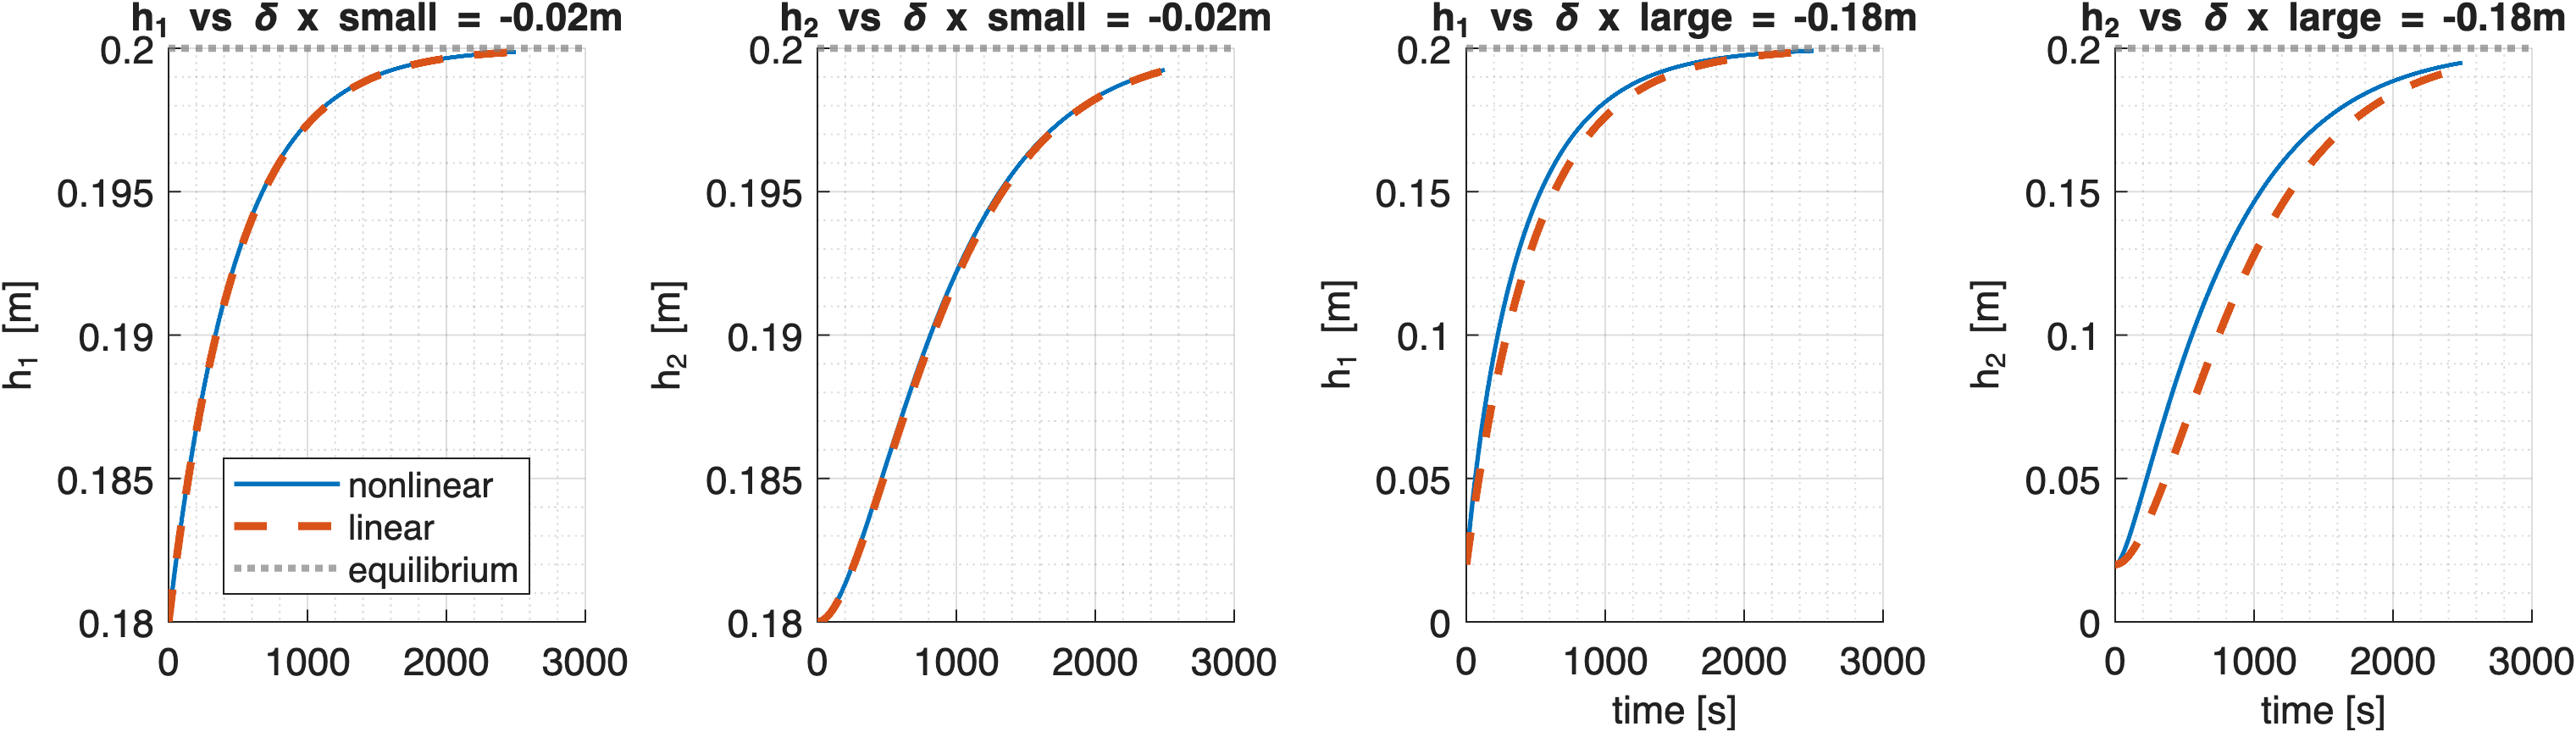
\includegraphics[width=16cm]{figures/q1_cmp}
    \captionof{figure}{Free response of the linearised and nonlinear 
    models under the constant equilibrium input, for different initial deviations. Far from the operating point the
    nonlinear response fills faster, as the linearisation overestimates the
    $\sqrt{h}$ outflow.}
    \label{fig:q1_cmp}
    \end{figpanelenv}
\end{figure}


The mechanism is more clear for $h_1$: the outflow velocity $\varphi(h) = \sqrt{2gh}$ is concave, so its tangent at the operating level lies above the true curve. The linearization therefore overestimates the outflow at low levels, since it enters negatively in $\dot h_1$. This overestimation makes the dynamics of the linear model lag behind. For $h_2$ it's more complicated, since the nonlinear term enters both positively and negatively, specifically, $\varphi_1$ enters positively and behaves as a inflow component, while $\varphi_2$ enters negatively and behaves as an outflow component. What matters is the impact that those non linear terms have in the overall linearization error, so we decompose their contribution to the overall linearization error. We start by restating the linear and non linear dynamics of $h_2$:

\begin{equation}
\dot h_2^{\text{lin}}
=\frac{1}{A_2}\Big[\,u_2 a_2\,\varphi_{\text{lin}}(h_1)
                   -u_3 a_3\,\varphi_{\text{lin}}(h_2)\,\Big],
\qquad
\dot h_2^{\text{nl}}
=\frac{1}{A_2}\Big[\,u_2 a_2\,\varphi_{\text{true}}(h_1)
                   -u_3 a_3\,\varphi_{\text{true}}(h_2)\,\Big],
\end{equation}
with $\varphi_{\text{true}}(h_i)=\sqrt{2g\,h_i}$. Subtracting term by term gives the two-channel error

\[
\begin{aligned}
\dot h_2^{\text{lin}} - \dot h_2^{\text{nl}}
&= \underbrace{\frac{u_2 a_2}{A_2}\,\big[\varphi_{\text{lin}}(h_1)-\varphi_{\text{true}}(h_1)\big]}_{\text{inflow-channel error, }\;e_{\text{in}}}
 \;-\; \underbrace{\frac{u_3 a_3}{A_2}\,\big[\varphi_{\text{lin}}(h_2)-\varphi_{\text{true}}(h_2)\big]}_{\text{outflow-channel error, }\;e_{\text{out}}} .
\end{aligned}
\]

Figure~\ref{fig:q1_decomp} shows this decomposition: the net error $\dot h_2^{\text{lin}}-\dot h_2^{\text{nl}}$ is an order of magnitude smaller than either errors, and it is negative. A negative net error means that the linear model fills $h_2$ more slowly than the nonlinear one, which is why the linear response of $h_2$ lags as well.




\begin{figure}[tb]
    \centering
    \begin{figpanelenv}{\linewidth}%
%
    \begin{subfigure}[t]{0.49\linewidth}
        \centering
        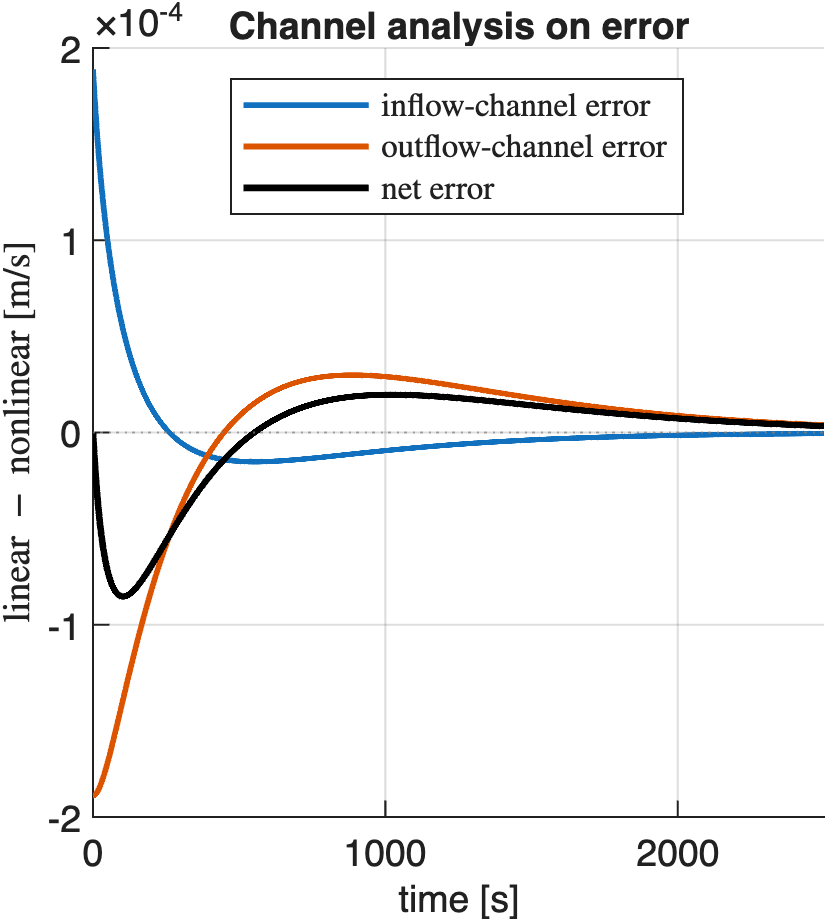
\includegraphics[width=4cm]{figures/q1_decomp}
        \caption{Error of $\dot h_2$ split into inflow ($+u_2a_2\varphi_1$)
        and outflow ($-u_3a_3\varphi_2$) channels.}
        \label{fig:q1_decomp}
    \end{subfigure}
    \hfill
    \begin{subfigure}[t]{0.49\linewidth}
        \centering
        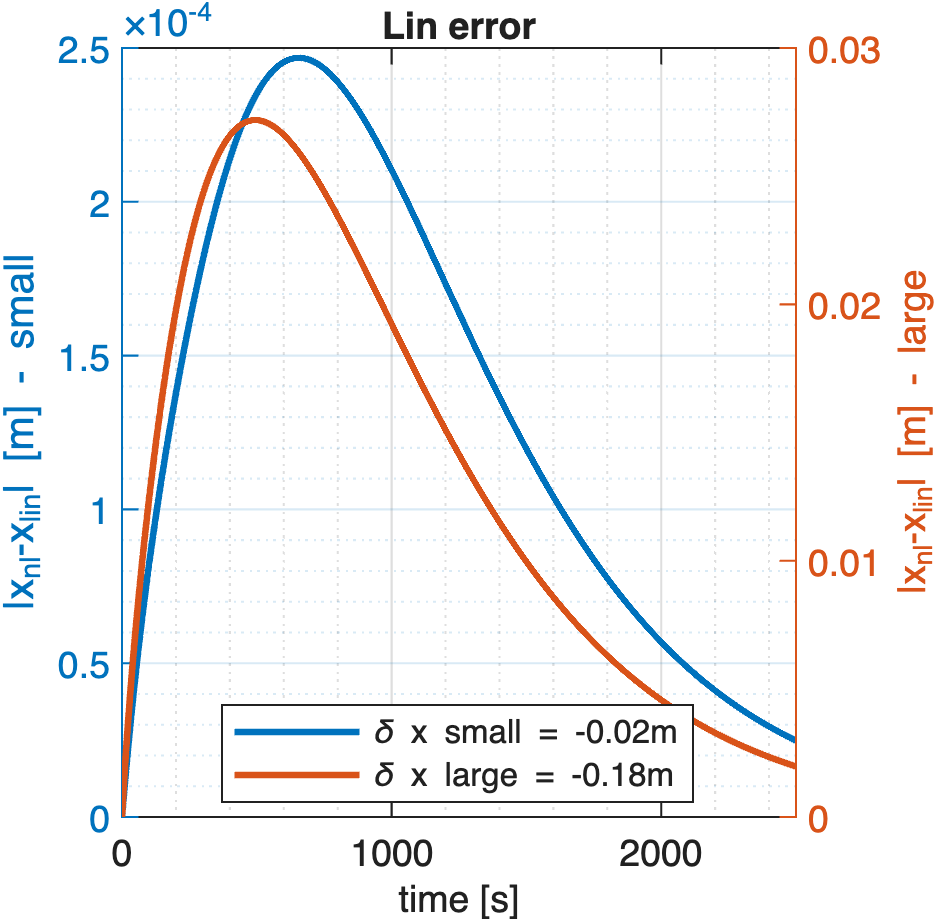
\includegraphics[width=5cm]{figures/q1_err}
        \caption{Norm of the mismatch
        $\|\bm{x}_{\mathrm{nl}}-\bm{x}_{\mathrm{lin}}\|$ for the two initial
        deviations (separate axes).}
        \label{fig:q1_err}
    \end{subfigure}
    \captionof{figure}{Linearization error. Channel decomposition~(a) and overall
    norm~(b); the peak scales by roughly two orders of magnitude between the
    small and large deviations.}
    \label{fig:q1_error}
    \end{figpanelenv}
\end{figure}

Figure \ref{fig:q1_err} quantifies the overall linearization error through $\| \bm x_{\text{nl}} - \bm x_{\text{lin}} \|$: the peak error goes from  $\approx2.5\times10^{-4}$~m for the small deviation to $\approx2\times 10^{-2}$~m for the large one -- roughly two orders of magnitude --
confirming that the linearization is accurate near $0.2$~m and degrades progressively as the state moves away from it.

\RuleSection{State-Feedback Design via LMIs}
\label{sec:q2}

With the plant linearised, we design a static state feedback $\delta \bm u = K \ \delta \bm x$ that makes the fluid level go back to the operating point. When applied to the plant, the command is: $\bm u = \bm{\bar u} + K(\bm{x} - \bm{\bar x})$. The feed-forward term $\bm{\bar u}$ sustains the equilibrium while $ K(\bm{x} - \bm{\bar x}) $ supplies the correction. The three gains obtained below rest on a common construction which is presented in this first section.

\subsection{From Lyapunov inequality to LMI}

The pair $(A,B)$ is controllable as $\operatorname{rank}[B \ AB] = 2 = n$, therefore its closed-loop eigenvalues can be assigned arbitrarily by state feedback. It's worth noting that the open loop is already asymptotically stable: state-feedback here it's not implemented to secure stability but to overcome the structurally slow response.  


In deviation coordinates the closed loop is $\quad \mathsf{d/dt} [\delta\bm{x}]
=(A+BK)\delta\bm{x}$, which is asymptotically stable if and only if $A+BK$
is Hurwitz, equivalently if there exists $P=P^\top\succ0$ such that
\begin{equation}
    \operatorname{He}\!\big(P(A+BK)\big)\prec0,\qquad
    \operatorname{He}(M):=M+M^\top.
    \label{eq:q2_lyap}
\end{equation}


Condition \eqref{eq:q2_lyap} is non linear because of the product $PBK$, and is therefore not a linear matrix inequality. Following \citep{zaccarian_lmi}, we can get to a linear LMI by the change of variables $W := P^{-1} \succ 0$: pre and post multiplying \eqref{eq:q2_lyap} by $W$ and setting $X := KW$ gives 


\begin{equation}
    W \succ 0, \qquad \operatorname{He}(AW + BX) \prec 0
    \label{eq:q2_baselmi}
\end{equation}

now linear in $(W,X)$. Any feasible pair recovers the controller and its
Lyapunov certificate as
\begin{equation}
    K=XW^{-1},\qquad P=W^{-1}.
    \label{eq:q2_recover}
\end{equation}

Controllability guarantees that \ref{eq:q2_lyap} has at least one solution, so a stabilizing $K$ always exists. 
%It's worth noting that there are no further requirements for the response 


\subsection{Arbitrary stabilizer}
\begin{wrapfigure}{r}{6.4cm}
    \centering
    \begin{figpanelenv}{6.4cm}%
%
    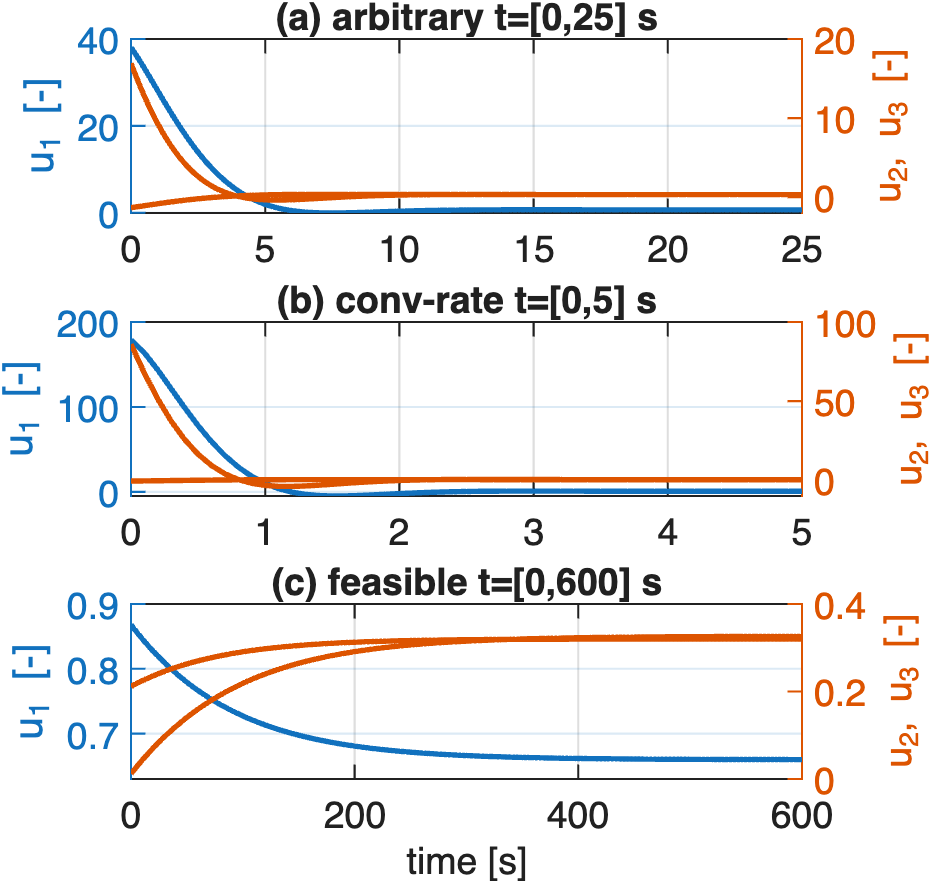
\includegraphics[width=5.7cm]{figures/q2_control}
    \captionof{figure}{Control signals for the three designs. Note: differing vertical
    scales, $u_1$ on the left axis and $u_2,u_3$ on the right. Different 
    time scales capture the transient.}
    \label{fig:q2_control}
    \end{figpanelenv}
\end{wrapfigure}
The first design solves the aforementioned problem in the previous section, with no objective nor constraints. At there there's no further optimization, the solver returns any arbitrarily feasible point. The found gain is $K_a$, which is available in the accompanying code. 

The following gain places the closed-loop eigenvalues at $\lambda_{1,2}(A+BK_a)=-0.500$. Simulated on the nonlinear plant, this gain drives the commands far outside the admissible range, as reported in (Table \ref{tab:q2_cmp}).


\subsection{Guaranteed convergence rate}
To command the speed of response we impose a certified convergence rate $\alpha$, by replacing~\eqref{eq:q2_baselmi} by \citep[eq.~(26)]{zaccarian_lmi}
\begin{equation}
    W\succ I,\qquad \operatorname{He}(AW+BX)\preceq-2\alpha W ,
    \label{eq:q2_lmi_b}
\end{equation}

where $\alpha$ is the exponential decay of the state norm $|\delta\bm{x}(t)|\le M\,e^{-\alpha t}|\delta\bm{x}(0)|$. The restrained normalization $W \succ I$ does not restrict feasibility and will be used in the next section.

Choosing $\alpha = \alpha_b = 2$ yields $K_b$, which is available in the accompanying code. It yields eigenvalues at $\lambda_{1,2}(A+BK_b)=-2.207$, which are smaller than the required $-2$ value imposed by the condition. The response is faster but the gain is an order of magnitude larger, thus the controls are even more out of bound. 

\subsection{Minimum-gain design with actuator authority}

The third design fixed the rate and minimizes a bound on the gain, so that the commands remain within the actuator range. 


Following
\citep[eq.~(27)]{zaccarian_lmi},
\begin{equation}
    \begin{aligned}
        \min_{W,X,\kappa}\quad & \kappa \qquad
        \text{s.t.}\quad & W\succ I,\qquad
            \operatorname{He}(AW+BX)\preceq-2\alpha W, \qquad
        & \begin{bmatrix} \kappa I & X^\top\\ X & \kappa I \end{bmatrix}\succ0 .
    \end{aligned}
    \label{eq:q2_lmi_c}
\end{equation}

A Schur complement on the last block gives $X^\top X \prec \kappa^2 \ I$, hence $\| X \| \le \kappa$; moreover, we have the condition that $W \succ 1$. These two conditions bound the gain $\| K \| = \|XW^-1\| \le \|X\| \le \kappa$. The rate has been manually tuned to $\alpha_c = 0.0115$, which makes sure that no control exceeds the bound $[0,1]$ on the nonlinear plant. The solution of the constrained optimization is reported in the accompanying code, and has eigenvalues at $\lambda_{1,2}(A+BK_c)=-0.0115=-\alpha_c$. Although its performances are far from the ones given by $Ka$ and $Kb$, one could appreciate through Table \ref{tab:q2_cmp} that the settling time is just $\approx 13\%$ of the uncontrolled settling time, which represents a sevenfold improvement on the open loop.

\subsection{Comparison}

Table \ref{tab:q2_cmp} has been produced in order to provide a quantitative evaluation of each gain's performance. 
Additionally, Figures \ref{fig:q2_state_short} and \ref{fig:q2_state_long} show the behaviour of the system with and without state-feedback: the first figure highlights the overshoot, while the second shows settling times of the slower dynamics. Finally, Figure \ref{fig:q2_control} shows the control trajectories using the three different gains. The best performance is provided by the second controller which employs $K_b$, while the controller which could be implemented in reality is the third one, although, as will be shown in the next sections, it's not robust to sensor failure. Using the third controller allows us to improve the open loop response by approximately seven times, while still respecting actuator feasibility. 

\begin{table}[htbp]
    \centering
    \small
    \renewcommand{\arraystretch}{1.1}
    \begin{tabular}{l r r r}
        \toprule
        Controller & $t_s$ [s] & $u_{\text{max}}$ & $u_{\text{min}}$ \\
        \midrule
        Open loop            & 2840 & 0.660 & \phantom{-}0.320 \\
        $K_a$ (arbitrary)    &    8 & 38.06 & --1.323         \\
        $K_b$ (rate)         &    2 & 178.99& --4.896          \\
        $K_c$ (min-gain)     &  385 & 0.868 & \phantom{-}0.012  \\
        \bottomrule
    \end{tabular}
    \caption{Closed-loop comparison on the nonlinear plant, from $\delta\bm{x}_0=-0.05$~m. Settling time $t_s$ is the time to enter and remain within $2\%$ of the initial step size; a $1.4$~s floor is applied to avoid the overshoot being mistaken for settling time. The commands of $K_a$ and $K_b$ leave the admissible range $[0,1]$, so their settling times are not physically realisable; only $K_c$ respects the actuator bounds. $u_{\text{max}}$ and $u_{\text{min}}$ are considered across all three controls. }
    \label{tab:q2_cmp}
\end{table}


\begin{figure}[tb]
    \centering
    \begin{figpanelenv}{\linewidth}%
%
    \begin{subfigure}[t]{6cm}
        \centering
        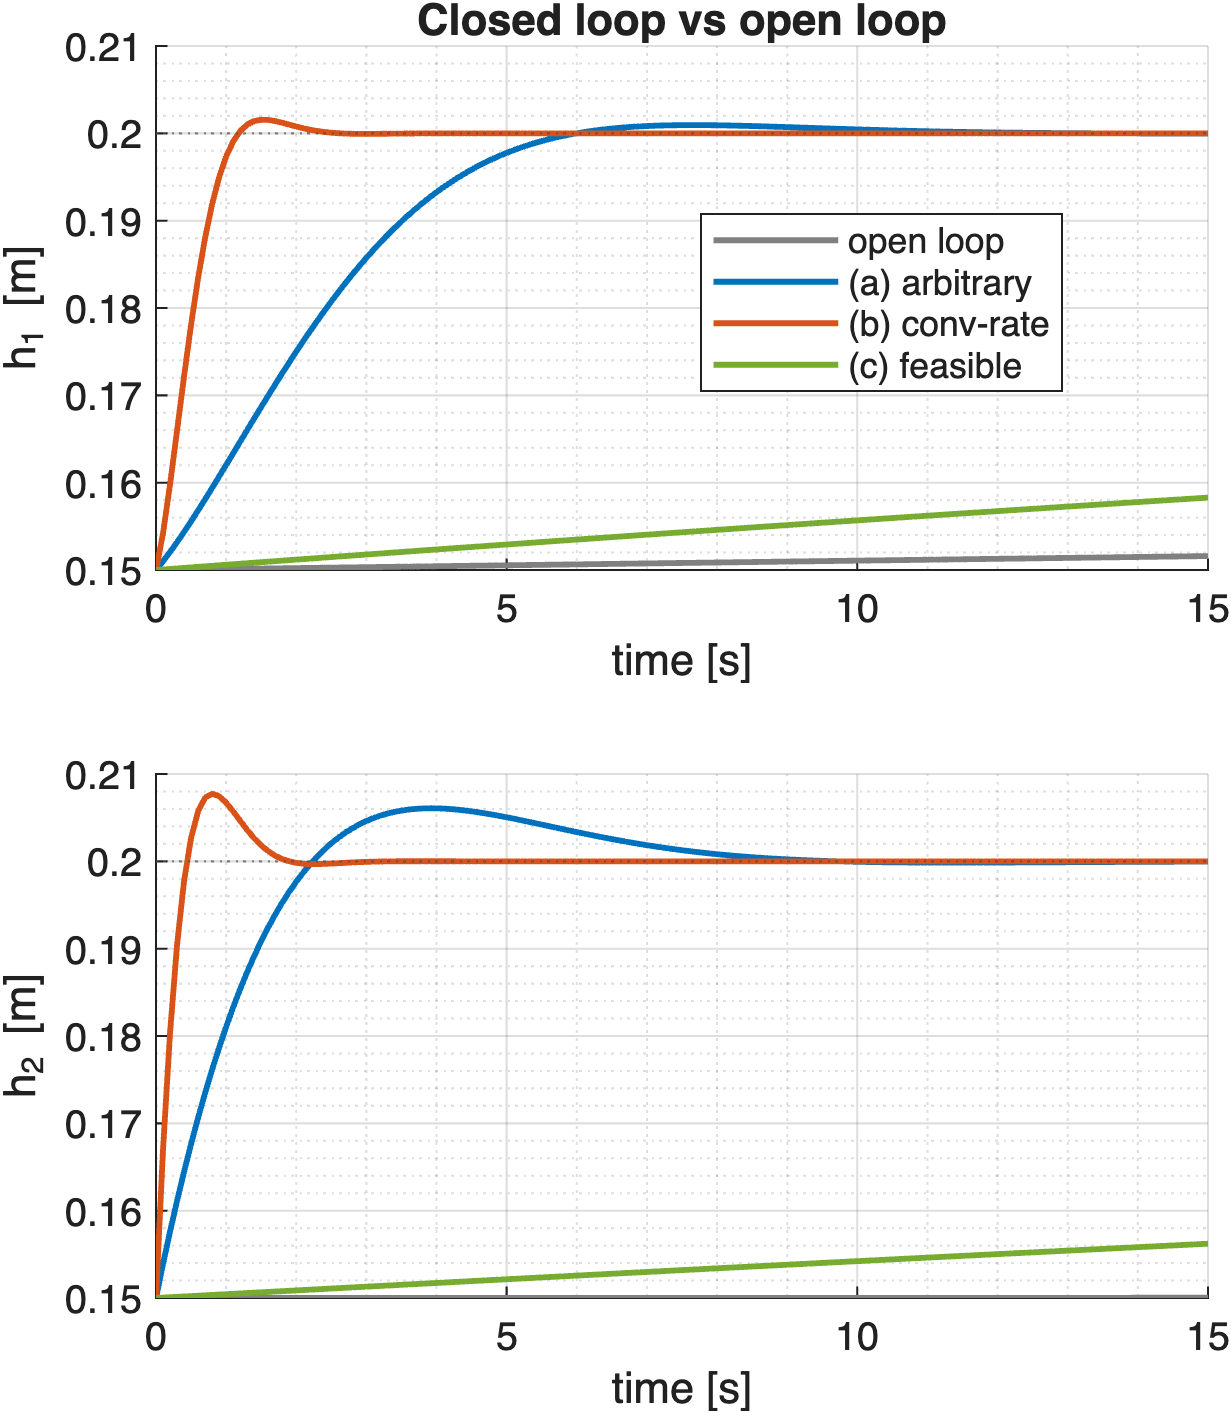
\includegraphics[height=7cm]{figures/q2_state_short}
        \caption{Short timescale ($0$--$15$~s): $K_a$, $K_b$ settle quickly
        but overshoot; $K_c$ rises gently.}
        \label{fig:q2_state_short}
    \end{subfigure}
    \hspace{2cm}
    \begin{subfigure}[t]{6cm}
        \centering
        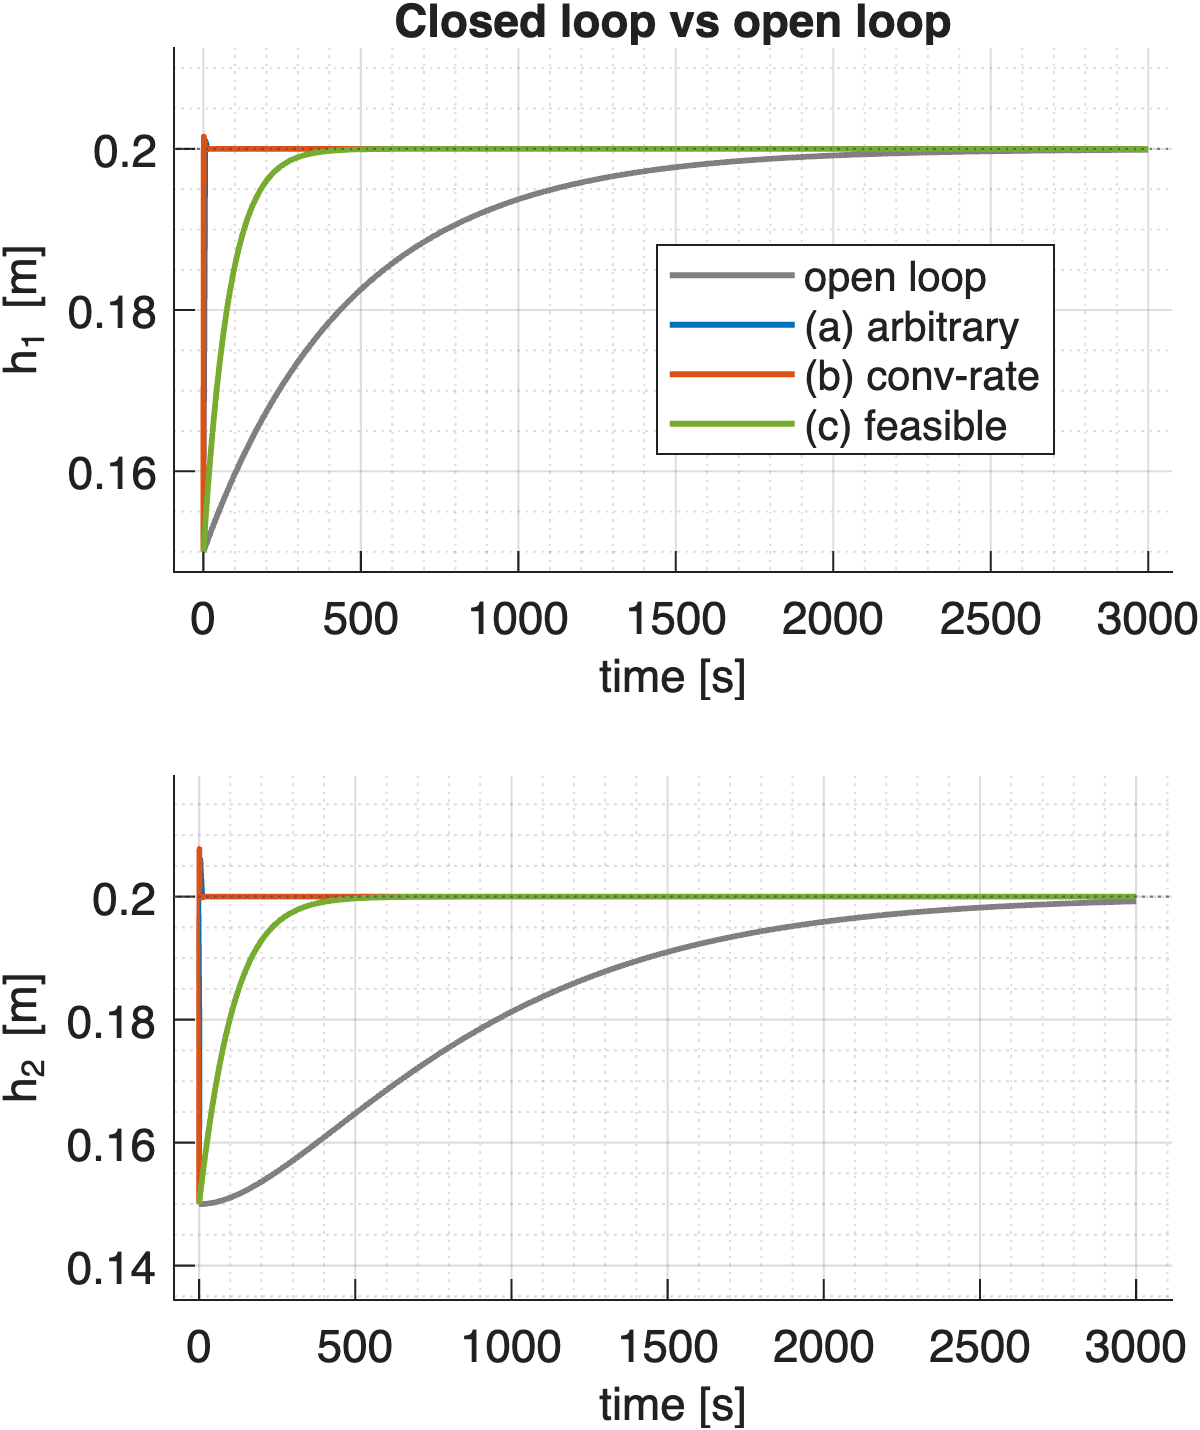
\includegraphics[height=7cm]{figures/q2_state_long}
        \caption{Full timescale ($0$--$3000$~s): $K_c$ settles in
        $\approx385$~s against the open-loop $\approx2840$~s.}
        \label{fig:q2_state_long}
    \end{subfigure}

    \captionof{figure}{Closed-loop state response on the nonlinear plant from
    $\delta\bm{x}_0=-0.05$~m, shown at two timescales. The apparent
    instantaneous settling of $K_a$ and $K_b$ in~(b) is obtained only with
    the inadmissible commands of Figure~\ref{fig:q2_control}.}
    \label{fig:q2_state}
    \end{figpanelenv}
\end{figure}



\RuleSection{Observer Design}
\label{sec:q3}

\subsection{Which sensor failure is recoverable}
If the sensor for $h_1$ fails, while sensor for $h_2$ remains functional, the matrix $C$ becomes $C_2 = [0\quad 1]$. In the other case, we'll have matrix $C_1 = [1\quad 0]$. For each case we can check whether the full state can still be recovered: i.e. whether the pair $(A,C_i)$ is observable. 

The observability matrix has rank $2$ for $C_2$ and rank $1$ for $C_1$. This tells us that a failure in sensor $h_1$ is recoverable while a failure in $h_2$ is not recoverable. The reason is the cascade structure of $A$. The matrix is lower-triangular, so $h_1$ does not depend on $h_2$ while $h_2$ does depend on $h_1$.  From now on, $\tilde C = [0 \quad 1]$.


\subsection{Observer gain}

The observer mirrors the model by working with a state estimate $\widehat{\delta \bm x}$. During its update, two components are summed together: the dynamics of the estimated state and a correction term, which depends on the difference among measured output and predicted output: 

\begin{equation}
    \mathsf{d/dt}\Big[\widehat{\delta\bm{x}}\Big]
    = A\,\widehat{\delta\bm{x}} + B\,\delta\bm{u}
      + L\,\big(\delta\bm{y}- \widehat y\big)
    = A\,\widehat{\delta\bm{x}} + B\,\delta\bm{u}
      + L\,\big(\delta\bm{y}-C\,\widehat{\delta\bm{x}}\big),
    \label{eq:q3_obs}
\end{equation}

The correction term is interesting as it is used as a proxy for the current "goodness" of our estimation. The matrix $L$ tells not only the sensitivity that the result has on the state, it also tells the direction in which the estimate should be corrected. 

Moreover, the estimation error $\bm{e}=\delta\bm{x}-\widehat{\delta\bm{x}}$ follows $\dot{\bm{e}}=(A-LC)\bm{e}$, therefore, we want $A-LC$ to have stable eigenvalues with a chosen rate, in order to have asymptotic stability towards zero. 

This is the dual of the state-feedback problem, because the estimation-error matrix $A-LC$ has the same eigenvalues as its transpose $(A-LC)^\top = A^\top - C^\top L^\top$. Assigning those eigenvalues by the choice of $L$ is therefore the same task as choosing a state-feedback gain for the pair $(A^\top,C^\top)$, which was exactly the problem of Section~\ref{sec:q2} with $A\to A^\top$ and $B\to C^\top$. Therefore, we solve the dual LMI:
\begin{equation}
    P\succ0,\qquad \operatorname{He}(PA-YC)\preceq-2\alpha_{\mathrm{obs}}P,
    \qquad L=P^{-1}Y .
    \label{eq:q3_lmi}
\end{equation}

With $\alpha_{\mathrm{obs}}=2$ the observer eigenvalues come out at $-3.254$ (both equal), well below the required $-2$. The estimate therefore converges much faster than the controller, whose eigenvalues are at $-0.0115$. It's worth noting that in this work we take the difference $A-LC$, meanwhile in \cite{zaccarian_lmi} the summation $A+LC$ is taken into consideration. Once the sign of the elements of $L$ are adjusted, the two formulations are equivalent.

\subsection{Estimation}

The observer is tested on the nonlinear plant with a sensor failure on sensor $h_1$. The initial deviation coordinates are $\delta \bm x = [-0.05, -0.05]$: $h_2$ is initialized at the correct value while $h_1$ is initialized at the equilibrium value $h_1(0) := h_1^{\text{eq}} = 0.2$.

Figure \ref{fig:q3_track} shows the result. The gain $\alpha_obs = 2$ dictates the kink in the trajectory at $t = 1.3s$: the trajectory then reaches within $1$ mm of true $h_1$ after $164.3$ s, as the tanks approach the operating point. The lag of the observer model is due to the fact that the observer is based on the linearised version of the model: if the observer is run on the linear state, the correction happens at $1.30$ s. 

\begin{figure}[tb]
    \centering
    \begin{figpanelenv}{\linewidth}%
%
    \begin{subfigure}[t]{0.49\linewidth}
        \centering
        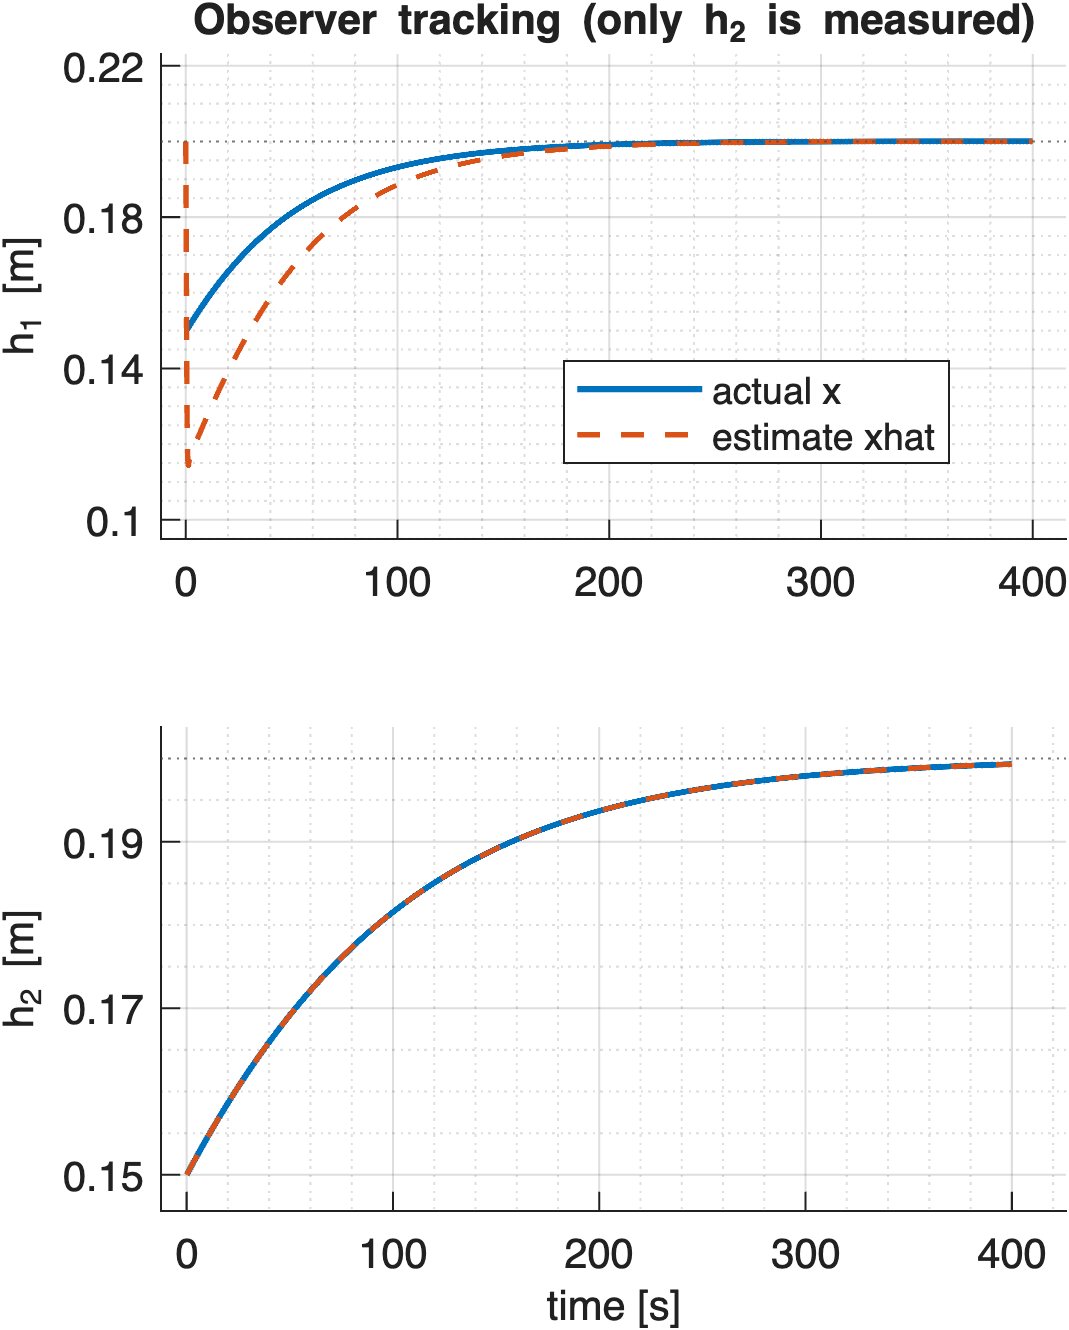
\includegraphics[height=7cm]{figures/q3_track}
        \caption{Observer estimate against the true state (only $h_2$
        measured). The $h_2$ estimate is exact from the start; the $h_1$
        estimate starts at $0.2$~m, dips near $t=1.3$~s, then converges.}
        \label{fig:q3_track}
    \end{subfigure}
    \hfill
    \begin{subfigure}[t]{0.49\linewidth}
        \centering
        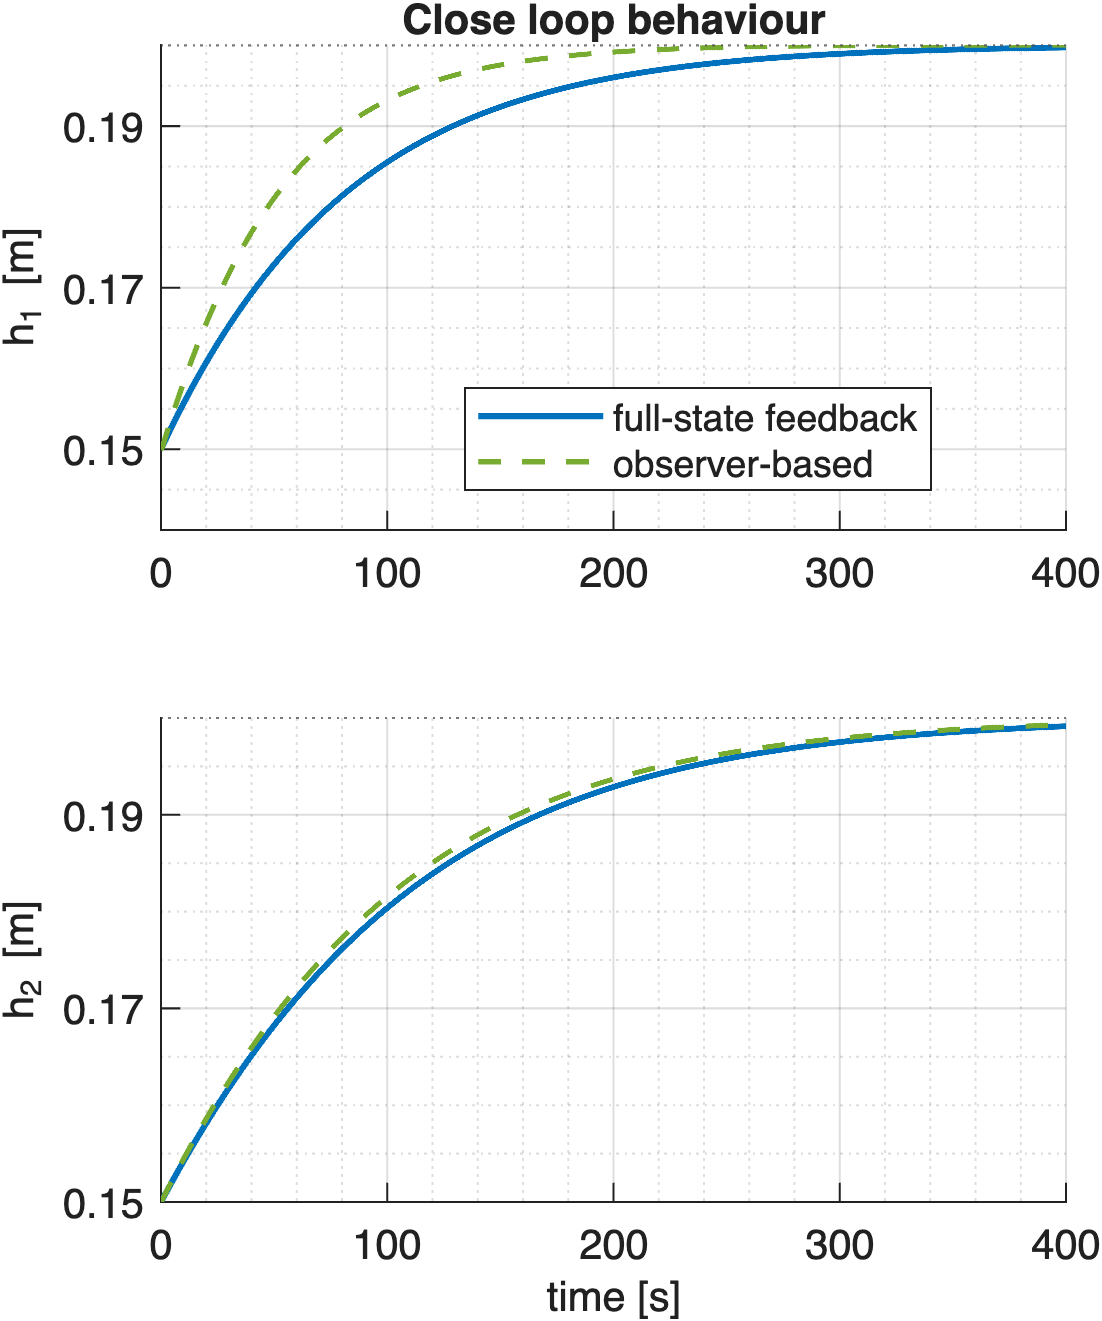
\includegraphics[height=7cm]{figures/q3_fb}
        \caption{Closed loop with true-state against observer-based feedback,
        both using $K_c$. Observer-based is slightly faster on $h_1$, then
        matches as the estimate becomes exact.}
        \label{fig:q3_fb}
    \end{subfigure}
    \captionof{figure}{Observer behaviour: state estimation~(a) and the resulting
    observer-based closed loop~(b).}
    \label{fig:q3}
    \end{figpanelenv}
\end{figure}


\section{Observer-based feedback}
With no $h_1$ sensor, the controller must use its estimate. By the separation principle the design splits in two. In the coordinates $(\delta\bm{x},\bm{e})$, where $\bm{e}=\delta\bm{x}-\widehat{\delta\bm{x}}$ is the estimation error, the closed-loop matrix is block-triangular, so its eigenvalues are those of the controller $A+BK_c$ together with those of the observer $A-LC$. The controller gives $\lambda_{1,2}=-0.0115$ and the observer gives $\lambda_{1,2}=-3.254$, so the closed loop has eigenvalues \footnotesize $\{-0.0115,\,-0.0115,\,-3.254,\,-3.254\}$, \normalsize that is, the union of the two sets: the system is therefore stable. The controller will now use $K_c$ from section \ref{sec:q2}.  The control law is:

\begin{equation}
    \bm{u}=\bar{\bm{u}}+K_c\big(\widehat{\delta\bm{x}}\,\big)
          =\bar{\bm{u}}+K_c(\hat{\bm{x}}-\bar{\bm{x}}).
    \label{eq:q3_fb}
\end{equation}

Figure \ref{fig:q3_fb} compares the observer-based loop with the full-state loop of section \ref{sec:q2}. Both reach the  operating point, although the observer based response is faster on $h_1$. The reason follows from Figure \ref{fig:q3_track}: $h_1$ is underestimated, driving the controller to fill more aggressively the first tank. 

Table \ref{tab:q3_cmp} makes the comparison precise: the observer-based loop settles faster on both tanks, although at the cost of actuators saturation. The smallest command drops to $-0.094$, which is outside of feasible range. A new gain $K_d$ is computed, in order to get a feasible gain compatible with the observation model distance from the real model. The manual tuning settles on $\alpha_d=0.0095$, a little below $\alpha_c$, which gives $K_d$. Its numeric value is available in the accompanying code. The associated eigenvalues are $\lambda_{1,2}=-0.0095$. 

The results of the simulation are stated in Table~\ref{tab:q3_cmp}: the controls are now feasible ($u_{\min}=0.004$), at the cost of a slower
response. Settling rises from $192$ to $255$~s on $h_1$ and from $367$ to $453$~s on $h_2$, about a third slower than the infeasible observer-based $K_c$.



\begin{table}[htbp]
    \centering
    \small
    \renewcommand{\arraystretch}{1.1}
    \begin{tabular}{l r r r r}
        \toprule
        Loop & \large $t_{s,h_1}$ \normalsize[s] & \large $t_{s,h_2}$ \normalsize [s] & $u_{\text{max}}$ & $u_{\text{min}}$ \\
        \midrule
        Full-state feedback ($K_c$)   & 303 & 385 & 0.868 & \phantom{$-$}0.012 \\
        Observer-based ($K_c$)        & 192 & 367 & 0.965 & --0.094         \\
        Observer-based ($K_d$)        & 255 & 453 & 0.891 & \phantom{$-$}0.004 \\
        \bottomrule
    \end{tabular}
    \caption{Full-state against observer-based feedback, both using $K_c$,
    from $\delta\bm{x}_0=-0.05$~m (same $1.4$~s settling floor as
    Table~\ref{tab:q2_cmp})}
    \label{tab:q3_cmp}
\end{table}

% ====================================================================== 
\bibliographystyle{abbrvnat}
\bibliography{references}   

\end{document}